
\subsection{Définitions et propritétés informelles}
\label{sec:informel}
% ⚠️ obsolète dû au remaniement des parties et annexes
% Commençons par introduire les données fonctionnelles de manière informelle afin de mieux intégrer la définition formelle, plus utile pour la manipulation.

Nous allons dans cette section introduire la notion de donnée fonctionnelle ainsi que les propriétés les plus utiles lorsqu'on les manipule. On y regroupe l'ensemble des messages essentiels à retenir des données fonctionnelles pour la pratique, sans alourdir les notions avec des notations mathématiques. Le cadre formel est traîté en annexe ~\ref{annexe:fda-formel}.

\begin{definition*}[données fonctionnelles — informel]
	Les données fonctionnelles sont des données dont les observations sont des fonctions, c'est-à-dire des courbes, des surfaces, des images, \, \dots

	i.e : toute donnée ayant une dépendance de type "relation fonctionnelle" avec un ou plusieurs paramètres.
	\label{def*:fda}
\end{definition*}

\begin{figure}[H]
	\begin{center}
		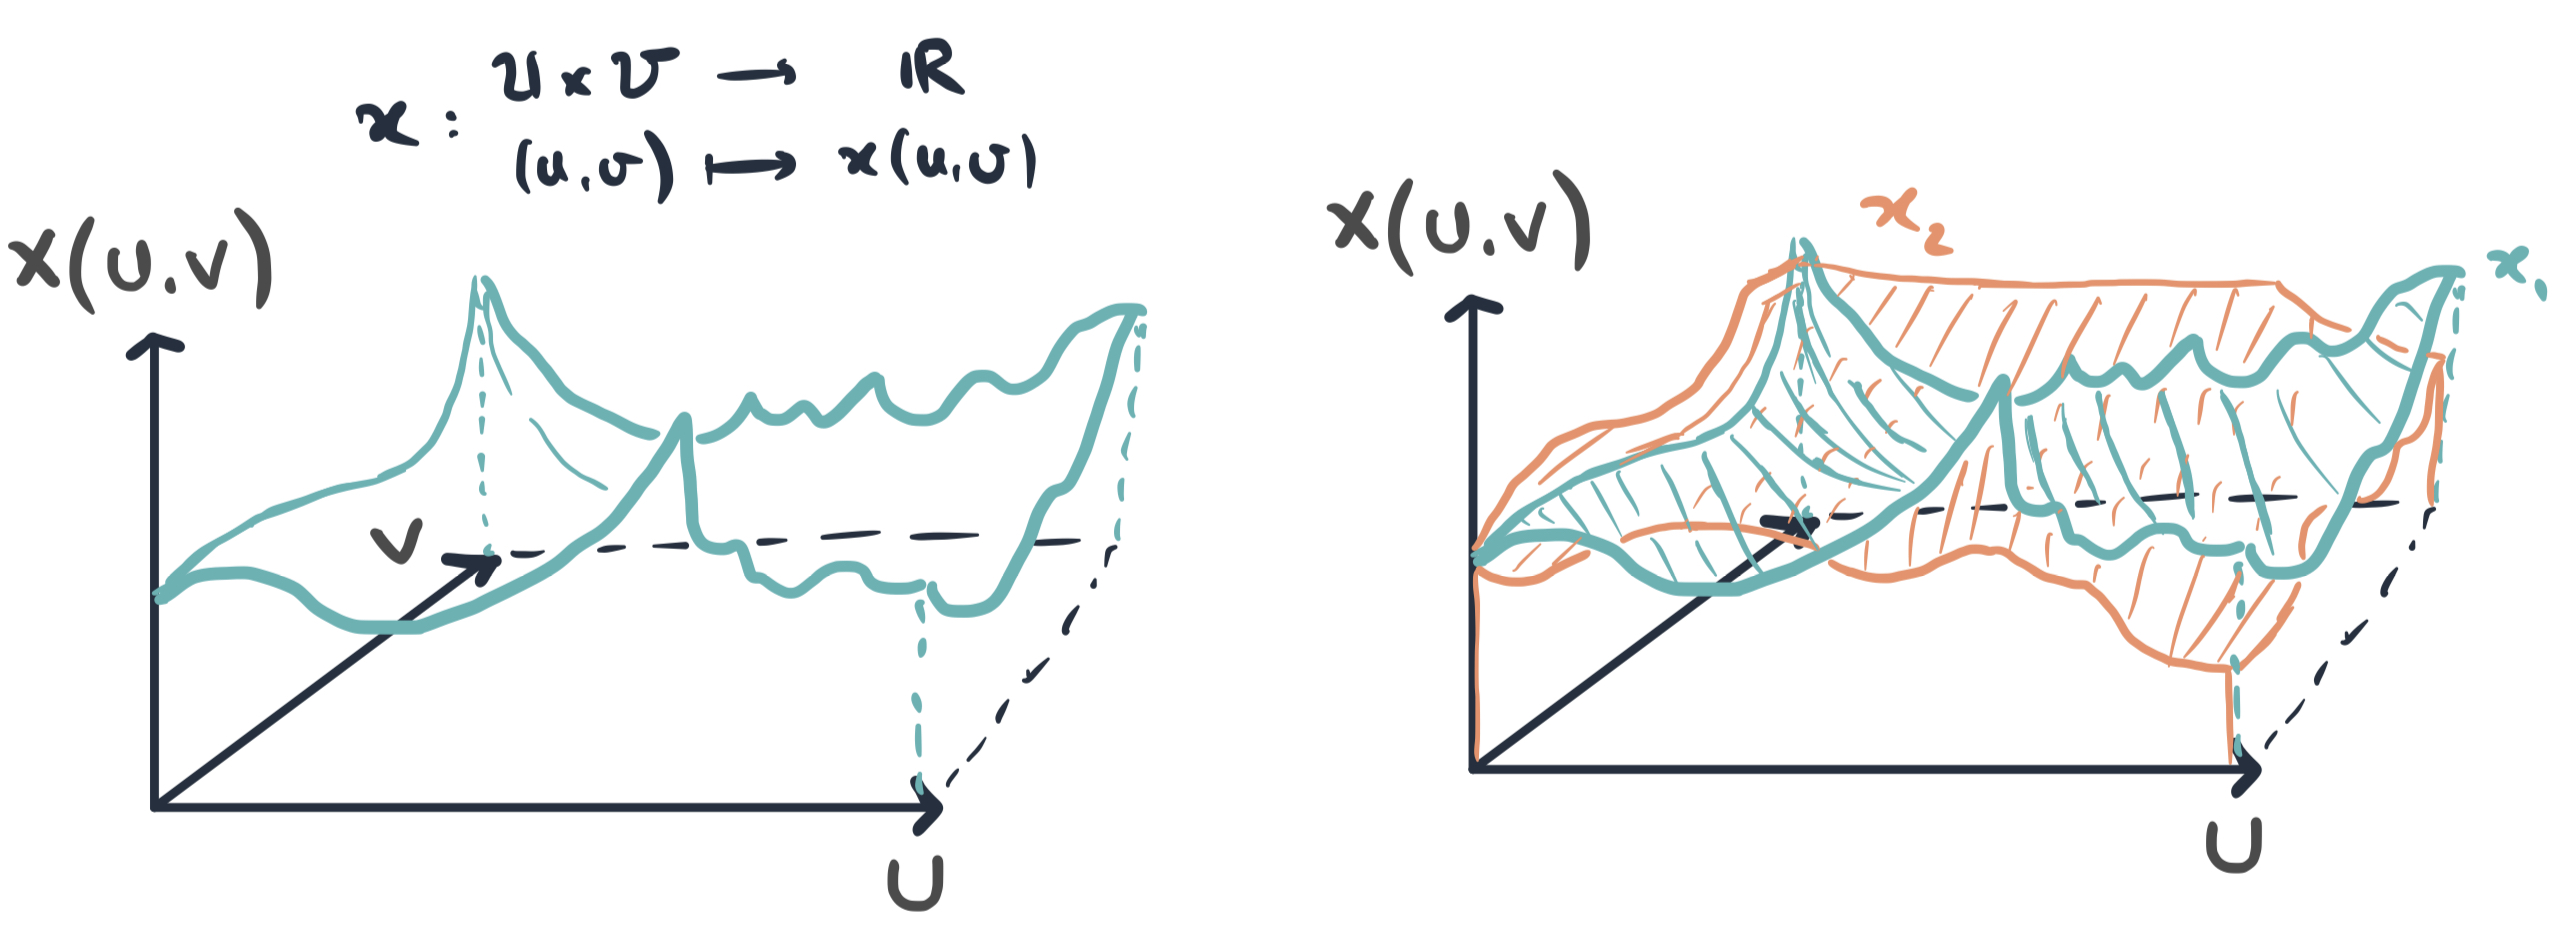
\includegraphics[width=0.8\textwidth]{Images/sketches/fda_surface.jpg}
	\end{center}

	{
	\textbf{Gauche :} exemple de surface
	\\
	\textbf{Droite :} échantillon de deux observations de la surface suivant une loi fonctionnelle}

	\caption{Donnée fonctionnelle : relation fonctionnelle avec plusieurs paramètres}
	\label{fig:sketch_surface}
\end{figure}

Maintenant introduites, les théorèmes suivant permettent de manipuler ces données à la fois pour la théorie et la pratique :

\begin{thm*}[\nameref{thm:KL} — informel]
	\noindent\fbox{%
		\parbox{\textwidth}{%
			Il est possible pour une large classe de données fonctionnelles de les décomposer dans une base \emph{de fonctions} adaptée aux données (au sens de la covariance) que l'on appelle base ACP fonctionelle (FPCA).
		}%
	}
	\label{thm*:KL}
\end{thm*}


\begin{rem}
	La classe de fonctions pouvant être décomposées est large, puisqu'elle regroupe l'ensemble des processus qui nous intéressent la plus part du temps en tant que statisticien : celles qui sont à support sur un intervalle, admettant une covariance continue et finie sur le support.
\end{rem}

On en déduit que pour travailler avec des données fonctionnelles, il suffit de les décomposer dans la base ACP fonctionnelle puis de travailler sur les composantes de chaque élément de la base. On travaille désormais avec des réels et non plus des fonctions, ce qu'on aime manipuler. On peut alors faire de la statistique traditionnelle avec les outils que l'on connait.


\begin{propriete*}[intérêt de la base FPCA — informel]
	\noindent\fbox{%
		\parbox{\textwidth}{%
			la base ACP fonctionnelle est la plus économe, c'est à dire qu'elle explique au mieux la covariance des données pour un nombre de composantes fixées, ce qui est utile car on ne sait manipuler numériquement que des objets de dimension finie.
		}%
	}
\end{propriete*}

Pour avoir une bonne représentation de ces données, on doit donc s'assurer de bien estimer la covariance. Pour cela, on a mentionné qu'il serait judicieux de lisser les observations en tenant compte de la régularité du processus dont est issu nos données. La question est désormais la suivante :

\question{
	Est-il possible de récupérer la régularité locale des trajectoires à partir des données ? Si oui, comment ?
}

C'est ce qu'affirme le théorème suivant provenant des travaux de Golovkine et MPV :

\bigskip

% TODO : créer un alias samepage 
% \samepage{stuff} = \noindent\begin{minipage}{\textwidth} stuff \end{minipage}
\noindent\begin{minipage}{\textwidth}
\begin{thm*}[Regularité locale — informel]
	\noindent\fbox{%
		\parbox{\textwidth}{%
			Les données fonctionnelles permettent de récupérer la régularité locale des trajectoires. Les estimateurs définis \textbf{ponctuellement} convergent.
		}%
	}
	\label{thm*:regularite_locale}
\end{thm*}
\end{minipage}
\begin{rem}[Continuité de Kolmogorov]
	Un théorème (\nameref{thm:kolmogorov_continuite}) permet à partir de l'espérance d'incréments d'un processus aléatoire de déduire sa régularité.
	C'est pourquoi les estimateurs sont définis à partir des incréments quadratiques. C'est entre autres \emph{la raison pour laquelle les données fonctionnelles permettent de récupérer la régularité locale des trajectoires}.

	\label{rem:kolmo_continuite}
\end{rem}


% \subsection{estimation adaptative informelle}
% Les motivations de l'obtention de la régularité étaient en partie de pouvoir mieux estimer les quantités qui nous intéressent dont la fonction moyenne du processus, ainsi que son opérateur de covariance. Ce qui est à la fois important pour l'analyse (via l'interprétation de la base ACP déterminée par la covariance) et pour la prédiction. On peut alors se demander si il existe des estimateurs de la moyenne et de la covariance prenant en compte la régularité locale. C'est ce qu'affirme les théorèmes suivants :

\warn{demander à Hassan la dernière version de son papier car la partie d estimation adaptative a beaucoup changé}

\begin{thm*}[Estimateurs de la moyenne et de la covariance — informel ~\cite{golovkine2021adaptive}]
	\noindent\fbox{%
		\parbox{\textwidth}{%
			Il est possible en lissant les observations par méthode à noyaux avec une largeur de bande \emph{spécifique à l'objet que l'on souhaite estimer}, de dériver des estimateurs de la moyenne et de la covariance qui convergent.
			La largeur de bande optimale \emph{pour l'objet que l'on souhaite estimer} est celle qui minimise un risque qui effectue un compromis biais-variance, qui dépend de la régularité locale du processus, en pénalisant les largeurs de bande menant à des "trous" dans les fonctions lissées.
			On parle d'\emph{\og estimation adaptative \fg}.
		}%
	}

	\label{thm*:estimation_adaptative}
\end{thm*}

Cependant, bien qu'une largeur de bande optimale existe, elle est inconnue. Il est donc important de savoir si le praticien peut l'estimer, et avec quelle précision (c'est à dire à quel point l'estimateur sera biaisé ou non). C'est ce que nous affirme le théorème suivant :

\begin{thm*}[expression de la largeur de bande optimale — informel ~\cite{golovkine2021adaptive}]
	\noindent\fbox{%
		\parbox{\textwidth}{%
			Sous certaines hypothèses de régularité du processus, et d'indépendance des temps observés, la largeur de bande optimale peut être approchée (avec forte probabilité de bonne approximation) par une expression ne dépendant que du nombre de courbes observées, du nombre moyen de temps observés par courbe, et de la régularité locale du processus. Ce biais de l'estimateur de la fonction moyenne est alors contrôlé en fonction de ces mêmes quantités.

			Sous des hypothèses un peu plus fortes sur la relation entre le nombre moyen d'observations par courbe et le nombre de courbes, on dispose de résultats similaires pour l'estimateur de la covariance.}%
	}

	\label{thm*:h_opt_estim}
\end{thm*}


Enfin, on peut se demander ce qu'il en est des estimateurs dans le cadre où l'on dispose de la dépendance dans les données (ce qui est la cas pour les données éoliennes notamment). Ce cas est traîté par le théorème suivant dérivé par MPV :

\begin{thm*}[ Estimation adaptative de séries temporelles fonctionnelles — informel ~\cite{maissoro-SmoothnessFTSweakDep} ]

	On peut estimer la régularité d'une série temporelle de données fonctionnelles à condition que la mémoire temporelle de la série soit courte. (La décroissance de la dépendance temporelle doit être au moins aussi rapide qu'une décroissance géométrique)

	\label{thm*:far_adaptative_estimation}
\end{thm*}

% \pagebreak

\subsection{Résumé de l'intérêt de la modélisation fonctionnelle}

Les données fonctionnelles permettent de travailler sur un modèle où la \emph{relation} entre plusieurs quantités est sujet à une loi \footnote{$cf$ \nameref{def*:fda} : \ref{def*:fda}}. Ce point de vue de réplication de courbes est notamment utile car il permet d'extraire des observations leur régularité\footnote{$cf$ \nameref{rem:kolmo_continuite}, \nameref{thm*:regularite_locale} : \ref{rem:kolmo_continuite}}. L'estimation de cette régularité permet, entre autres, de lisser les courbes de façon appropriée en fonction de la quantité que l'on souhaite estimer, telle que la moyenne et la covariance avec une plus grande précision\footnote{$cf$ \nameref{thm*:estimation_adaptative} : \ref{thm*:estimation_adaptative}}.

\noindent\begin{figure}[H]
	\centering
	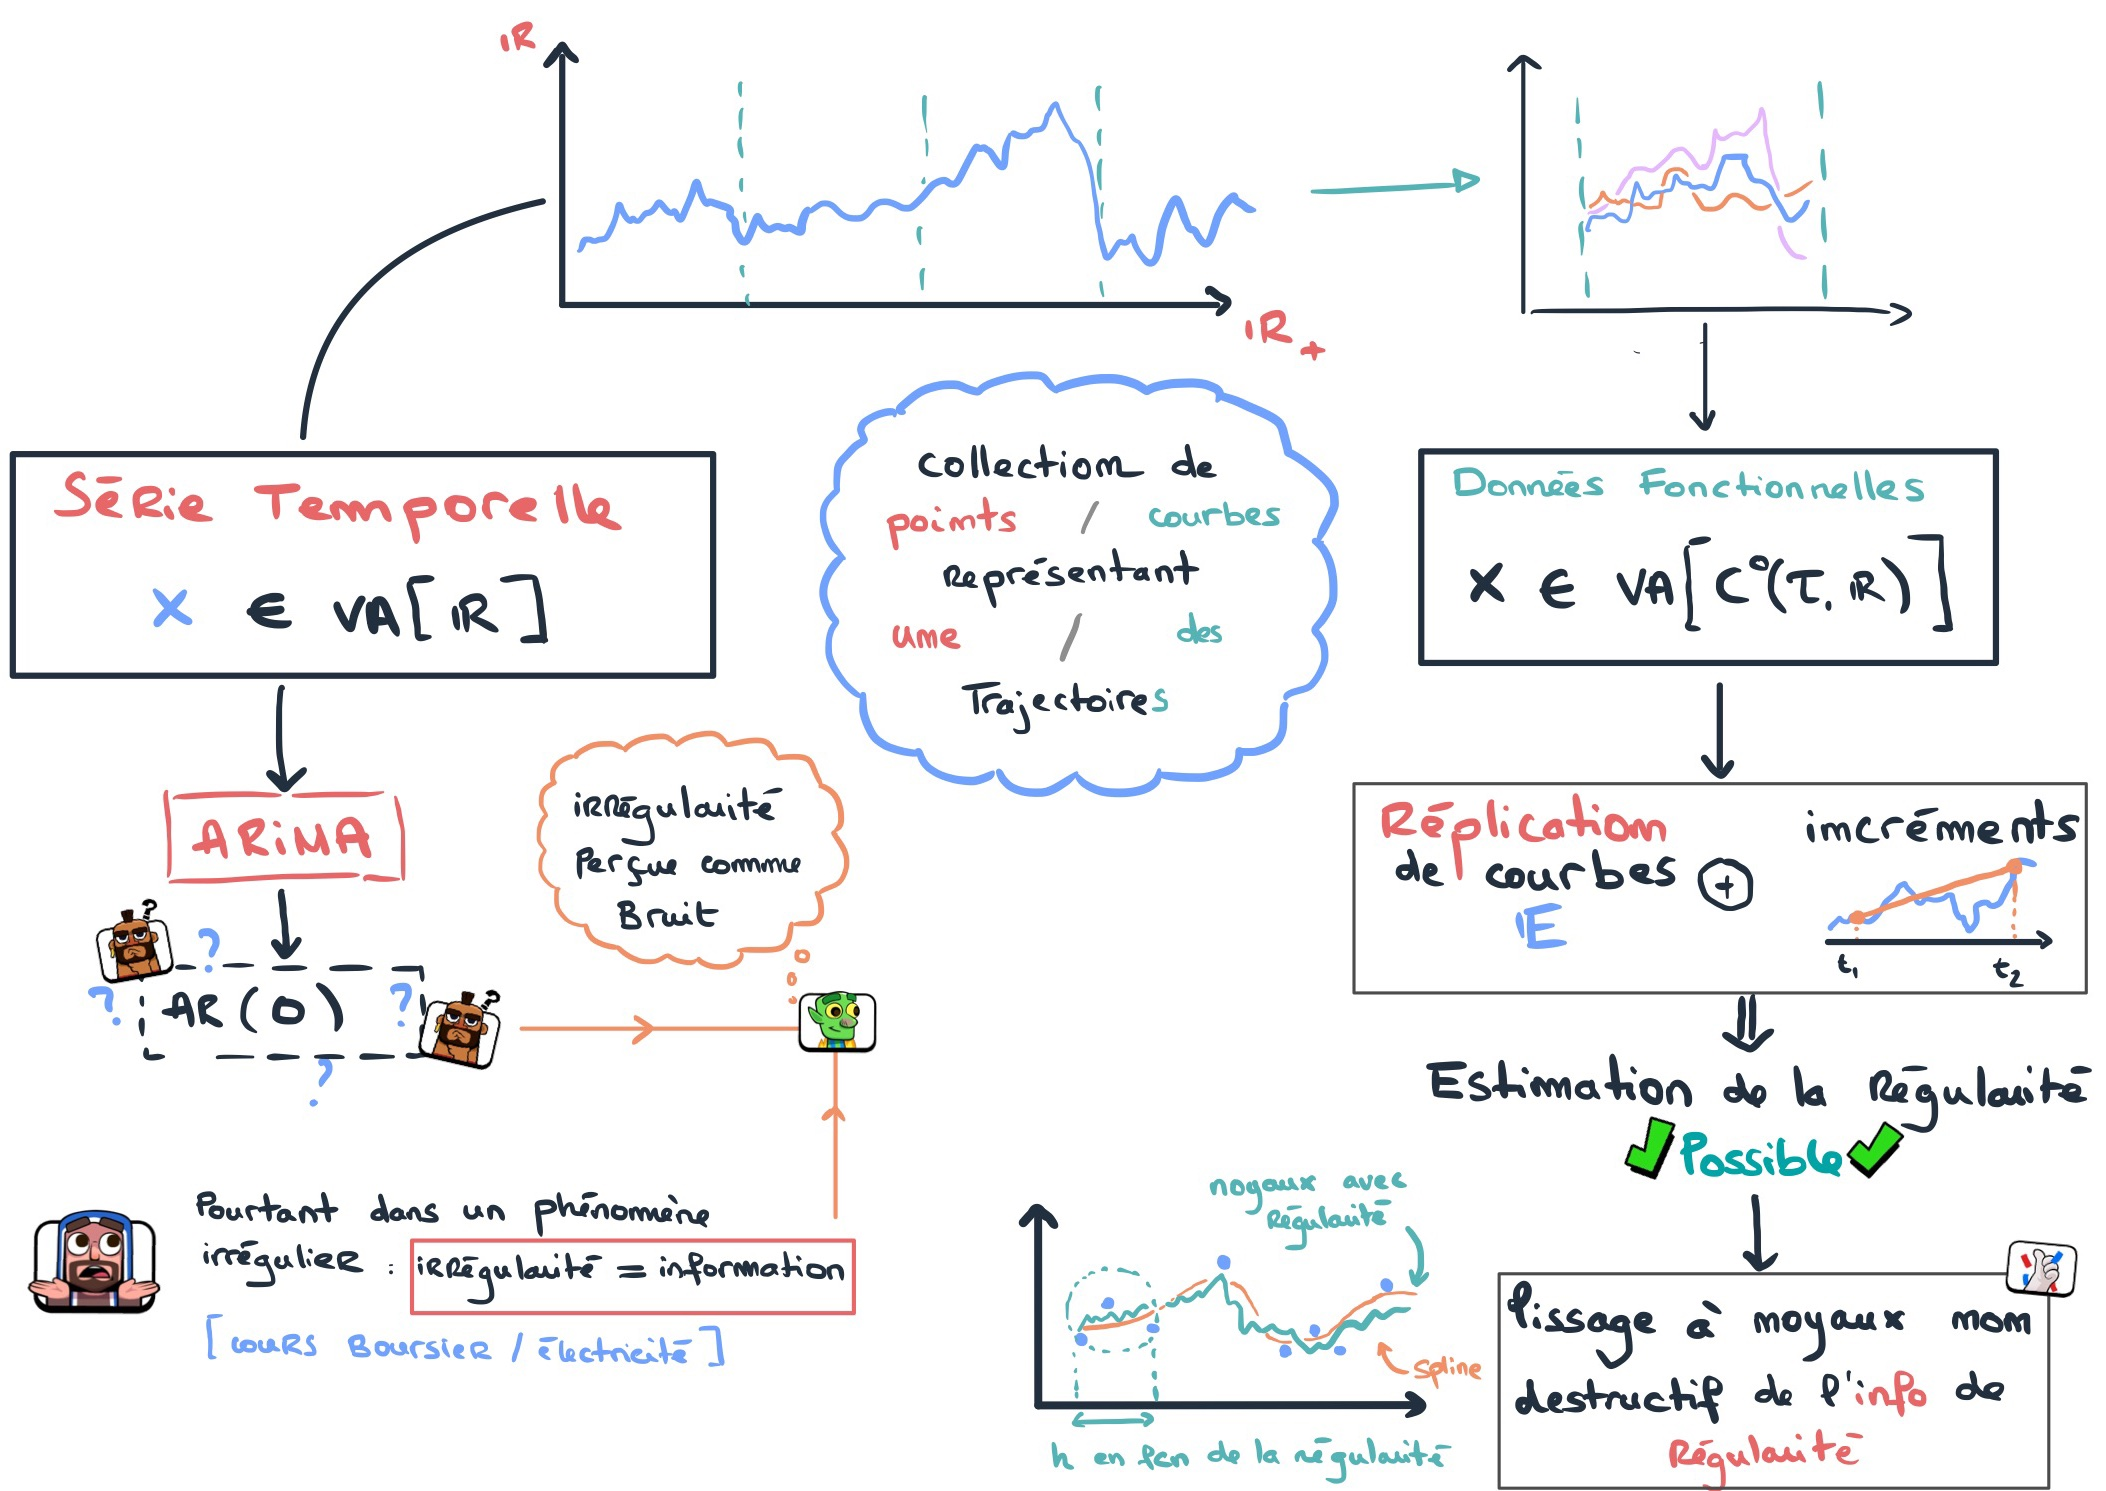
\includegraphics[width=0.8\textwidth]{Images/sketches/sketch_resume_informel.jpeg}
	\caption{Résumé des motivations du de l'estimation de la régularité locale des trajectoires}
	\label{fig:sketch_resume_informel}
\end{figure}

\pagebreak

% \subsection{Données fonctionnelles : formellement}
% \subsubsection{Définition formelle}

Pour éviter d'alourdir les notations, on se place dans le cas où les fonctions sont à valeurs dans $\mathds R$ et à support sur un intervalle fermé $I$ de $\mathds R$. Toutefois, on peut très bien considérer des fonctions à valeurs dans $\mathds R^d$ et à support sur un compact $K$ de $\mathds R^p$ sans perte de généralités.

\begin{definition}[données fonctionnelles ]

    On appelle données fonctionnelles, un échantillon $\famfinie x 1 n$ de fonctions continues $x_i : I \rightarrow \R d$ issues d'un processus $X$ défini comme ci-dessous :

    $$X :
        \begin{array}{ccc}
            \Omega & \longrightarrow & \mathcal C(I, \mathds R)
            \\
            \omega & \longmapsto     & X(\omega) = x
        \end{array}
    $$

\end{definition}

\subsubsection{Résultats importants}

On énonce désormais le théorème central de l'analyse de données fonctionnelles qui n'est autre que la décomposition dans la base FPCA de notre processus.

\begin{rem}
	on notera que dans le cadre des données fonctionnelles, on ne travaille pas de façon générale avec la covariance :

	$$C_X : (s,t) \mapsto \esperance{ \left[X - \mu\right](s) \cdot \left[X - \mu\right](t) }$$

	On travaille plutôt avec l'\textbf{opérateur} de covariance :

	\begin{equation*}
		c : \begin{array}{ccc}
			\mathds L^2 & \longrightarrow & \mathds L^2                             \\
			f           & \longmapsto     & \int\limits_I f(u)C_X(u, \cdot \,) \,du
		\end{array}
	\end{equation*}

	C'est parceque cet opérateur est linéaire continu (car Hilbert-Schmidt donc borné pour la norme d'opérateur) symétrique semi-défini positif (pour le produit scalaire de $\mathds L^2$) et que l'on peut donc en faire une décomposition spectrale sur une base orthonormale de vecteurs propres associés à des valeurs propres positives. Cette décomposition est à la base des approximations que le praticien effectuera ainsi qu'à la base de la dérivation de nombreux théorèmes et propriétés.
\end{rem}

\bigskip

Etant donné que l'on traîte des données fonctionnelles, on considère la géométrie usuelle de $\mathds L^2(\mathds R, \, \lambda)$ et on note ainsi

\begin{equation*}
	\prodscalselon \cdot \cdot {\mathds L^2}: \begin{array}{ccc}
		\mathds L^2 \times \mathds L^2 & \longrightarrow & \mathds R
		\\
		(f,g)                          & \longmapsto     & \int f(u)g(u) \, d\lambda(u)
	\end{array}
\end{equation*}


le produit scalaire que l'on considère pour manipuler les données fonctionnelles.


% https://stackoverflow.com/a/4008463 : no page break
\begin{minipage}{\textwidth}
	\begin{thm}[Karhunen-Loeve]
		\emph{référence :} ~\cite[pages : 238-239-241]{kokoszka2017introduction}

		\textbf{Hypothèses :}

		\begin{equation*}
			\boxed{
				\begin{array}{ll}
					\textsf{\faCaretSquareRight} & X \in \mathds L^2( \Omega, \mathcal C(I, \mathds R))
					\\ \\
					\textsf{\faCaretSquareRight} & \textsf{covariance : } C : \begin{array}{ccc}
						                                                          \mathds L^2( \Omega, \mathcal C(I, \mathds R)) & \longrightarrow & \mathcal C(I^2, \mathds R)
						                                                          \\
						                                                          X                                              & \longmapsto     & C_X
					                                                          \end{array}
					\\ \\
					                             & \textsf{ie : } C_X : (s, t) \mapsto C_X(s,t) \textsf{ est continue}
					\\ \\
					\textbf{\faIcon{asterisk}}   & \textsf{opérateur covariance} \, c_X[ \, \cdot \, ] : \begin{array}{ccc}
						                                                                                     \mathcal C(I, \mathds R) & \longrightarrow & \mathcal C(I, \mathds R)
						                                                                                     \\
						                                                                                     f                        & \longmapsto     & \int_I f(s) C_X(s, \cdot \, ) \, ds\end{array}
					\\\\
					\textsf{\faCaretSquareRight} & \textsf{valeurs propres ordonnées : } \forall p \geq 1, \lambda_{p+1} \leq \lambda_p \quad\quad \lambda_p, \lambda_{p+1} \in \operatorname{sp}(c_X)
					\\ \\
					\textbf{\faIcon{asterisk}}   & \textsf{on pose } \overrightarrow{sp}_{\orthonormal}^{[1,p]}(c_X) \isdef \left\{ \phi_k \in \overrightarrow{sp}_{\orthonormal}( \, c_X \, ) \textsf{ associé à }  \lambda_k, k \in \intervaleint 1 p \, \right\}
				\end{array}
			}
		\end{equation*}

		\textbf{alors :}
		\begin{equation*}
			\boxed{
				\begin{array}{cc}
					\textsf{\faCaretSquareRight} &

					\forall p \geq 1
					\quad
					\argmin\limits_{u_k \in \mathcal C(I, \mathds R)} \mathds E \left\Vert X - \sum\limits_{k=1}^p \prodscalselon {X - \mu} {u_k} {\mathds L^2} u_k \right\Vert^2 = \overrightarrow{sp}_{\orthonormal}^{[1,p]}( \, c_X \, )

					\\
					\\
					\textsf{\faCaretSquareRight} & X = \mu + \sum\limits_{k=1}^{+\infty} \prodscal {X - \mu} {\phi_k} \phi_k
					\\
					                             &
					\\
					                             & \textsf{avec } \phi_k \in \overrightarrow{sp}_{\orthonormal}( \, c_X \, )
				\end{array}
			}
		\end{equation*}

		\label{thm:KL}
	\end{thm}
\end{minipage}
\begin{proof}[\faCogs \, preuve informelle]
	La covariance est un opérateur bilinéaire symétrique défini positif, on peut donc appliquer le théorème de Mercer (équivalent du théorème spectral) qui nous donne une base orthonormale de $\mathds L^2$ sur laquelle on va décomposer notre processus \textbf{centré}.
\end{proof}


\begin{rem}
	pour pouvoir ordonner les valeurs propres dans l'ordre décroissant, et sélectionner les composantes principales les plus informatives, il faut pouvoir réarranger l'ordre de la somme. Pour cela il faut que les valeurs propres forment une famille sommable, une condition suffisante et souvent utilisée est que $\mathds E \Vert X \Vert^2 < \infty$
\end{rem}

\begin{rem}
	la propriété de la section précédente sur l'aspect économe de la base FPCA découle directement de l'assertion
	\begin{equation*}
		\forall p \geq 1
		\quad
		\argmin\limits_{u_k \in \mathcal C(I, \mathds R)} \mathds E \left\Vert X - \sum\limits_{k=1}^p \prodscal {X - \mu} {u_k} u_k \right\Vert^2 = \overrightarrow{sp}_{\orthonormal}^{[1,p]}( \, c_X \, )
	\end{equation*}
	dans le théorème de Karhunen-Loeve.
\end{rem}



% \pagebreak

\subsection{Cas non indépendant : séries temporelles de données fonctionnelles}
Une large partie de la théorie des données fonctionnelles suppose que l'on observe des courbes $X_i : \Omega \rightarrow \mathcal C^0(I, \mathds R)$ \textbf{indépendantes} et identiquement distribuées. Cependant une partie non négligeable des données que l'on observe ont des dépendances avec les valeurs passées. Par exemple, il est raisonnable de penser que la consommation électrique d'un foyer au cours d'une année croît avec l'ajout successif de nouveau appareils électroniques. L'hypothèse d'indépendance entre les données n'est donc plus pertinente pour les données que l'on traite et il devient important de considérer des processus autorégressifs adaptés aux données fonctionnelles.
Si dans le cadre des données de $\mathds R$ cette relation de \emph{dépendance linéaire} avec le passé pouvait s'écrire sous la forme suivante
$X_n = \sum\limits_{k=1}^{n-1} \varphi_k \, X_k + \xi_n$ où $\varphi_k \in \grandR$
et
$\xi_n \begin{cases} \in \operatorname{VA}(\grandR) \\ \indep \sigma\left( X_i \right)_{1\,: \, n-1}\end{cases}$,
dans le cadre fonctionnel on capture la même idée en considérant
$X_n = \sum\limits_{k=1}^{n-1} \phi_k \left( X_k \right) + \xi_n$ où $\phi_k$
est un \emph{opérateur linéaire} de $\mathds L^2(I, \mathds R)$,
le plus souvent intégral.

\chk{
	Il s'agit d'une généralisation naturelle de la relation dans le cadre réel, puisqu'on peut démontrer que sur l'espace des nombres réels l'ensemble des fonctions linéaires $\phi : \grandR \rightarrow \grandR$ sont de la forme $x \mapsto ax$ avec $a \in \grandR$. La relation sur $\grandR$ que l'on a vue juste avant peut alors se ré-écrire de façon similaire à la version fonctionnelle.
}

On considère lors de ce stage des séries temporelles de données fonctionnelles car les données que l'on manipule ( en l'occurence les données de courbe de charge des parcs éoliens ) semblent être naturellement corrélées dans le temps.


\question{Pourquoi se soucier en particulier des séries temporelles fonctionnelles lorsque l'on souhaite incorporer la régularité du processus dont est issu nos données dans l'estimation des quantités qui nous intéressent ?}

Rappelons-nous que les données fonctionnelles sont la clé pour déterminer la régularité, et que cela est en réalité permis par le théorème de \nameref{rem:kolmo_continuite} (que nous n'avons pas énoncé en détails, mais mentionné dans la section \ref{sec:informel}). Malheureusement, dans le monde réel où vit le praticien, nous n'avons pas accès à l'espérance de la loi dont sont issues nos données. Il nous faut donc estimer cette espérance, et c'est là que les séries temporelles fonctionnelles entrent en jeu. Puisque l'estimateur usuel de l'espérance est la moyenne empirique, qui nous est fourni par la loi des grands nombres, cela devient très problématiques lorsque l'on dispose de données corrélées.
% TODO ✏️ mieux formuler - dépendance faible -> LGN faible -> estim esperance
Ce que nous allons voir, c'est que l'on peut tout de même utiliser l'estimateur usuel de l'espérance, et que l'on obtiendra des estimateurs des paramètres de régularité convergents ponctuellement vers ceux du processus dont sont issues nos données. Ce résultat est dérivé en utilisant une forme particulière de dépendance que le lecteur pourra étudier plus en détail en annexe \ref{annexe:regularite-locale}.

\begin{figure}[H]
	\centering
	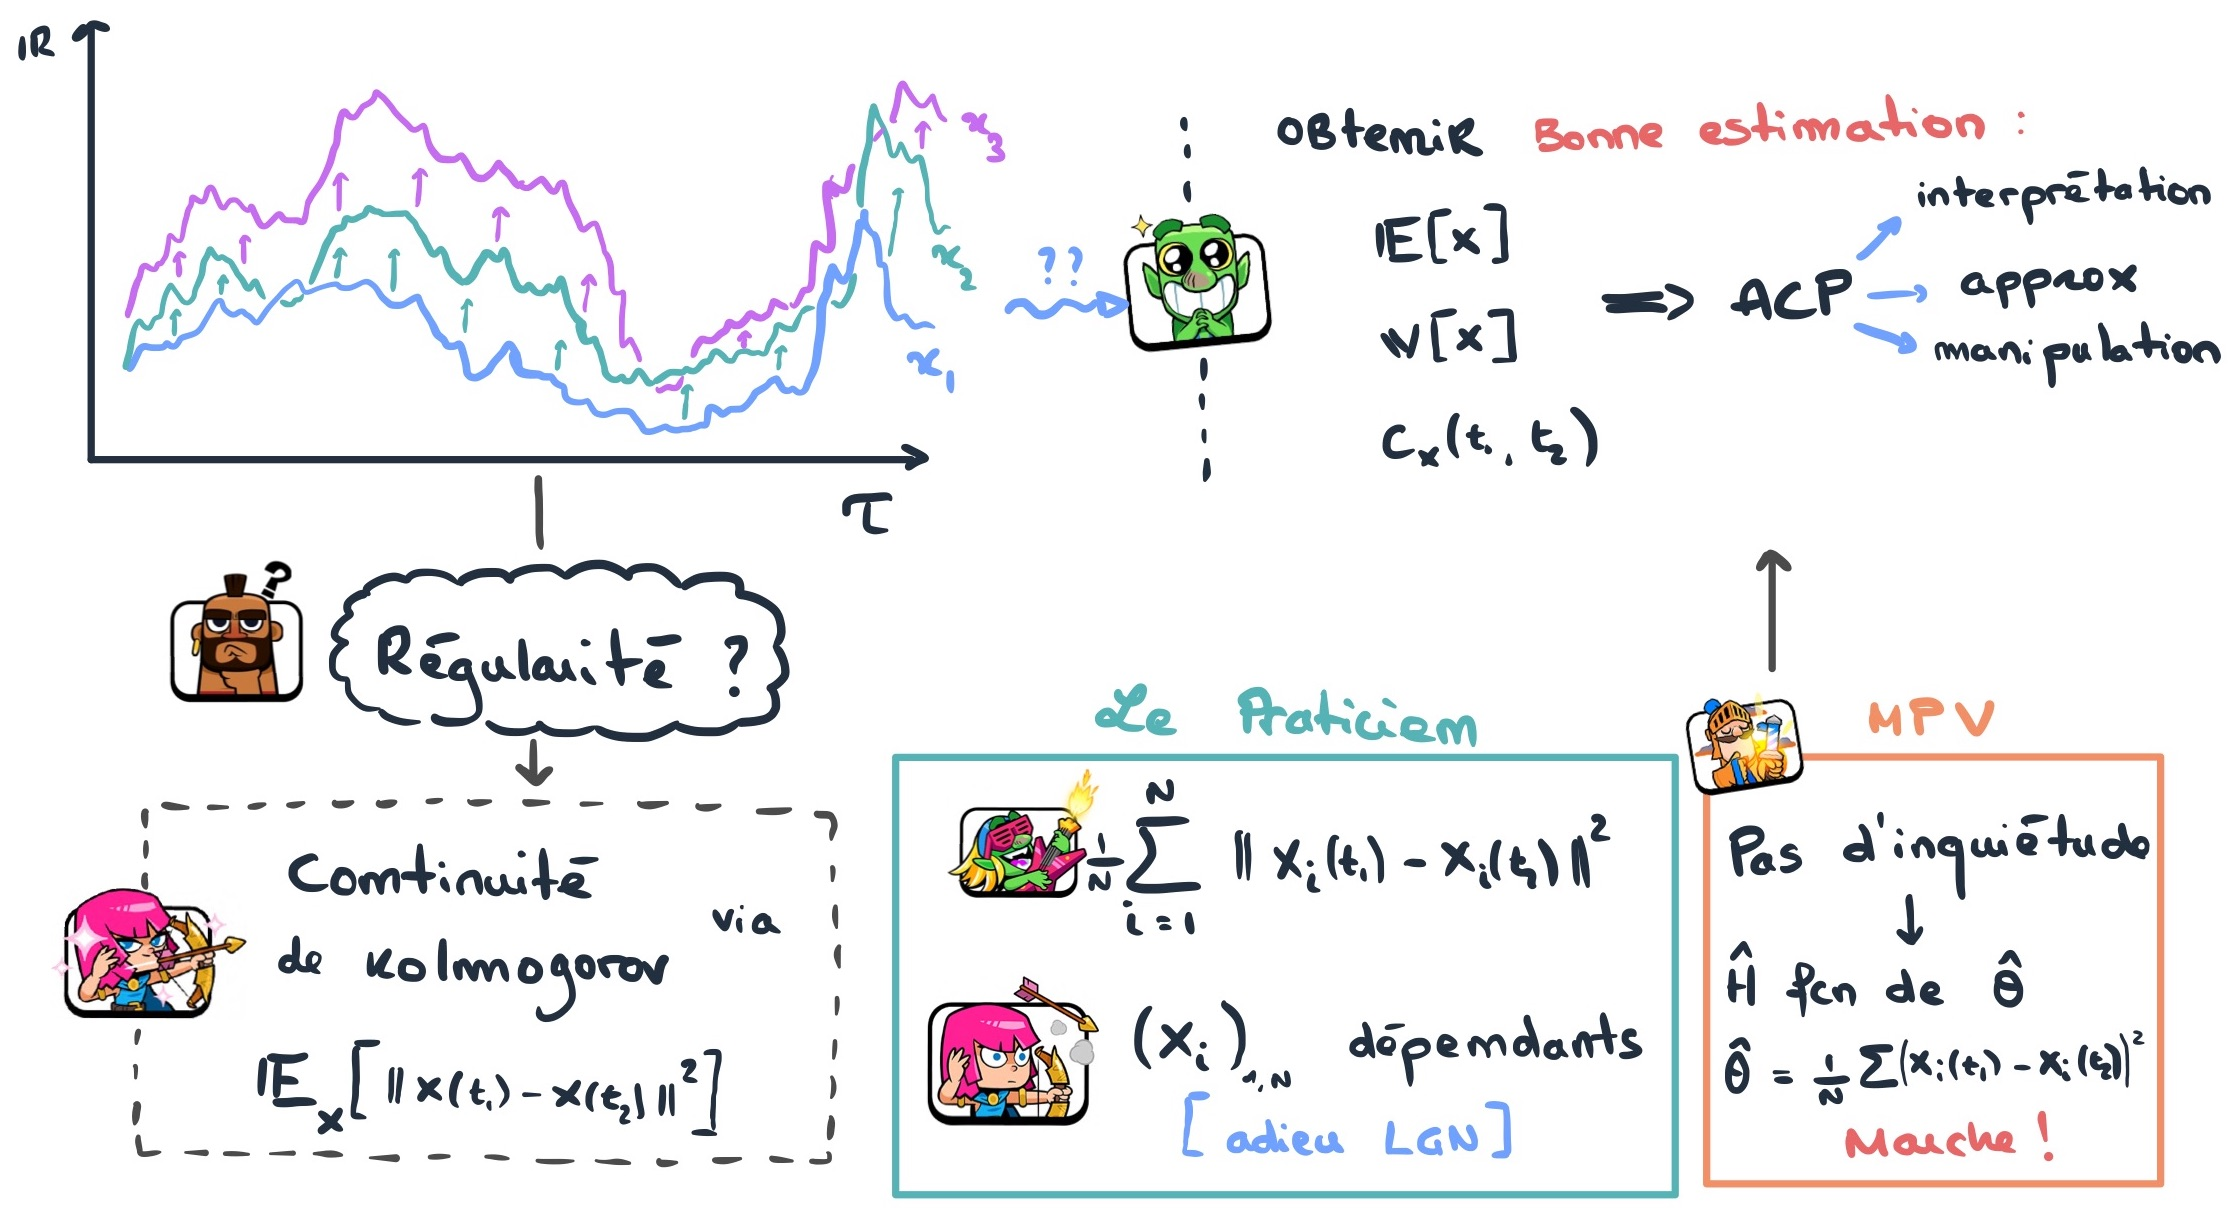
\includegraphics[width=\textwidth]{Images/sketches/schema_ts_estim_reg.jpg}
	\caption{Schéma grossièrement récapitulatif : Estimation de la régularité pour une série temporelle fonctionnelle}
	\label{fig:recap_estim_reg_fts}
\end{figure}


\warn{Il faut faire attention lorsque l'on manipule ou interprète des séries temporelles fonctionnelles. (comme par exemple tout résultat utilisant la loi de $\sum\limits_n X_n$, ... )}

Une série temporelle discrète est le fait que l'observation suivante dépend linéairement de l'observation précédente, dans le cadre fonctionnel \emph{l'observation est une fonction}. La dépendance se fait sur l'indice de la fonction, et non pas sur l'argument de la fonction interprété dans notre caps comme étant le temps.

\bigskip

Dans le cadre éolien c'est d'autant plus trompeur de parler de temps car on observe des courbes de charge sur une année : à la fois l'indice de la fonction et l'argument de la fonction ont des interprétations temporelles.

\smallskip

\noindent\fbox{%
    \parbox{\textwidth}
    {%
        dans l'expression \og$X_n(t)$\fg, la série temporelle (discrète) concerne bien l'indice $n$ et non pas l'argument $t$.
    }
}

\bigskip

\noindent La question devient alors :
\question{Lorsque l'on a une dépendance dans les observations fonctionnelle $\left\{ X_1 \dots X_n \right\}$, possède-t-on une dépendance dans les observations ponctuelles à $t$ fixé $\left\{ X_1(t) \dots X_n(t) \right\}$ ? Cette dépendance est-elle la même ?}

\noindent Et la réponse, c'est qu'\textbf{on ne sait pas}. En tout cas, dans le cadre général. Il y a en effet plusieurs façon de définir ce qu'on appelle par \og dépendance temporelle \fg. Toutes les définitions de dépendance ne mènent pas à cette conclusion, mais celle adoptée par (MPV) l'est, étant plus faible. De manière générale, lorsque l'on traîte des données avec de la dépendance, il convient d'être extrêmement précautionneux avec les théorèmes et \og faits \fg que l'on invoque. Toujours bien vérifier les hypothèses.

\bigskip
\noindent\fbox{\parbox{\textwidth}{%
		\noindent La dépendance faible comme définie dans l'article de MPV\cite{maissoro-SmoothnessFTSweakDep} nous permet de travailler localement : On peut travailler localement sur les trajectoires tout en utilisant des hypothèses fonctionnelles (que ce soit pour la dépendance ou autres) pour obtenir la régularité.}}

\input{content/chapter_2/01-fda_essentiel/03-time_series/01-03-simulation.tex}
\pagebreak
